\chapter[Software]{Software}
    

    \section[WebService]{WebService}

        A demanda do problema exige que diferentes hardwares se integrem com uma
        mesma base de dados. Fundamentalmente, o Smartphone do usuário realiza a compra, e
        o token deve reconhecer o QrCode para que o usuário consuma o chopp.
        
        Para solucionar essa demanda foi proposto uma arquitetura orientada a serviços
        (SOA), tal que uma webservice REST seja responsável pela persistência e autenticação de todos os
        dados relevantes do sistema, incluindo a autenticação de pagamentos.

        A tecnologia escolhida para implementação desse sistema foi o framework o 
        Ruby On Rails\footnote{\url{http://rubyonrails.org/}}, pela facilidade no desenvolvimento, 
        ampla comunidade e experiência da equipe. Sendo o Ruby na versão 2.3.0 e o Rails na versão 5.0.5.

        Para autenticação de pagamentos foi utilizada a API do PagSeguro\footnote{\url{https://github.com/pagseguro/ruby}},
        que recebe as requisições do WebService com os dados do comprador e registra a transação caso os dados estejam corretos,
        ou retorna erros, caso contrário. Quando o pagamento dessa transação muda de status, ou seja, é aprovado, o PagSeguro
        manda uma notificação de volta para o WebService de modo que assim possa ser gerado o QRCode.

        A persistência dos dados ocorre seguindo o modelo abaixo:

        \begin{figure}[H]
            \centering
            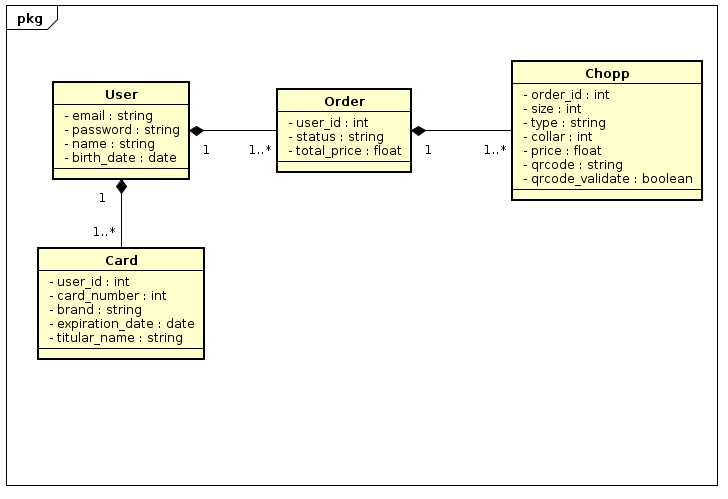
\includegraphics[scale= 0.4]{figuras/Diagrama-de-classes.png}
            \caption{Modelagem. Fonte: Própria.}
            \label{modelagem}
        \end{figure}

        Para hospedagem do WebService foi usado o Heroku\footnote{\url{https://www.heroku.com/}}.
        As vantagens em utilizar essa plataforma estão no custo, 
        por ser uma ferramenta grátis e na facilidade de fazer o deploy.

    \section[Sistema De Compras]{Sistema De Compras}

    O Sistema de Compras é composto de um app que será utilizado por
    quem deseja comprar um chopp. O comprador, ao utilizar o app, deve selecionar as preferências 
    em relação ao chopp e após essa etapa, inserir os dados do cartão de crédito para efetuar o pagamento. 
    Uma vez efetuado o pagamento, o sistema emitirá um código QR que deverá ser lido pela máquina
    para liberação do chopp.

    Esse sistema se comunica com o WebService citado anteriormente através de
    requisições GET e POST. Sendo assim, todo dado que precisa ser persistido ou recuperado é feito através
    dessas requisições.

    Para o desenvolvimento do app foi utilizado o framework Ionic. Esse framework
    nos permitiu uma maior produtividade visto que podemos desenvolver um app multi-
    plataforma que atende tanto a plataforma Android quanto IOS. 

    Abaiixo estão listados as telas do aplicativo:

    \begin{figure}[H]
        \centering
        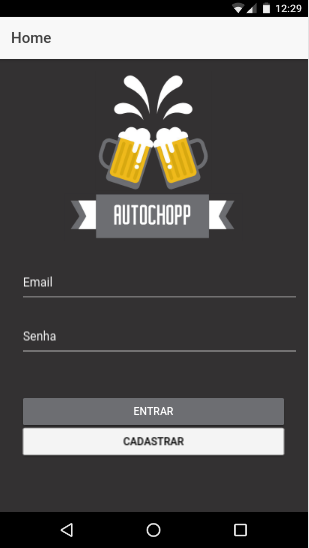
\includegraphics[scale= 0.4]{figuras/homepage.png}
        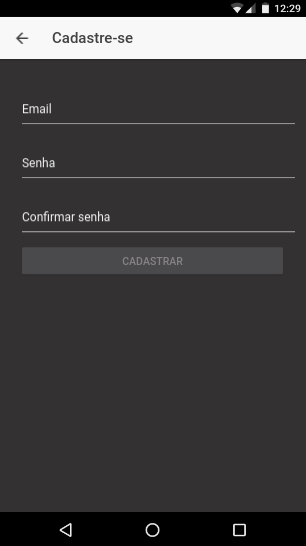
\includegraphics[scale= 0.4]{figuras/signup.png}   
        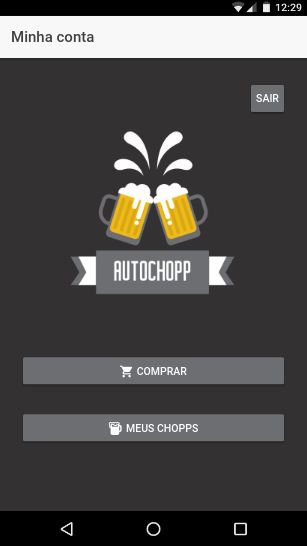
\includegraphics[scale= 0.4]{figuras/home-loged.png}
        \caption{Página Inicial - Registrar - Página Inicial com usuário logado. Fonte: Própria.}
        \label{telasapp1}
    \end{figure}

    \begin{figure}[H]
        \centering
        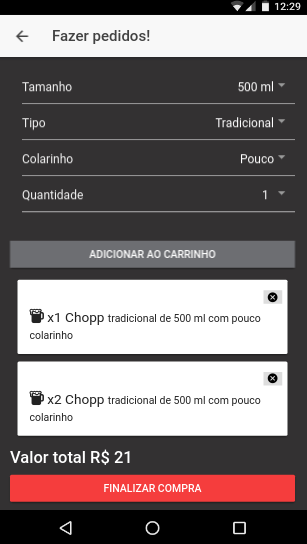
\includegraphics[scale= 0.5]{figuras/pedidos.png}        
        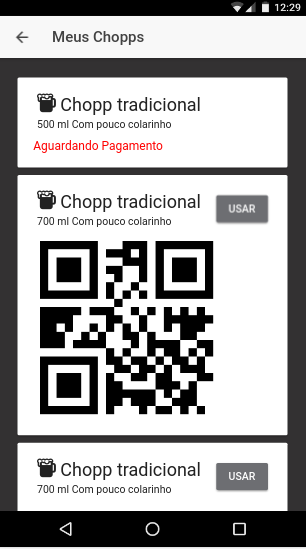
\includegraphics[scale= 0.5]{figuras/MeusChopps.png}
        \caption{Tela de Compra - Tela de Pedidos. Fonte: Própria.}
        \label{telasapp2}
    \end{figure}


    \section[Sistema Administrativo]{Sistema Administrativo}

        O Sistema administrativo está incorporado ao aplicativo do Sistema de Compras, porém apenas usuários
        administradores possuem acesso. Ao utilizar o aplicativo, o usuário visualiza
        as seguintes informações referentes ao estado da máquina: a quantidade de chopp que a
        máquina possui, a temperatura de resfriamento e o status da conexão da máquina com a internet.

        Esses valores são recuperados através de requisições GET ao WebService que guarda essas informações recebendo
        requisições POST a cada 60 seg da aplicação que lê os dados dos sensores. 
    
    \section[Sistema de Validação de Compra]{Sistema de Validação de Compra}
        
        O sistema de validação se trata do módulo responsável pela validação dos dados da compra,
        e dar o inicio no processo de serventia de chopp conforme as característias são pré-definidas.
        Esse subsistema tinha como resultados esperados uma aplicação que pudesse prover ao usuário
        a leitura do \textit{QRCode} gerado no momento da compra do chopp por meio de uma câmera 
        acoplada na máquina de onde o chopp é armazenado. No \textit{QRCode} estão contidas as informações
        referentes as preferências do consumidor no que tange sua bebida.
        
        Devido à necessidade de que o usuário tenha acesso a uma câmera para leitura do \textit{QRCode},
        foi escolhido o \textit{framework} Python Kivy\footnote{\url{https://kivy.org/}} por fornecer um ambiente
        \textit{touchscreen} com um baixo consumo de recursos, uma vez que essa aplicação estará 
        instanciada em uma Raspberry responsável por gerenciar outros módulos operacionais do projeto.

        Desta forma, foi então desenvolvida aplicação Autochopp-Machine \footnote{\url{https://github.com/autochopp/autochopp-machine}} que fornece de forma interativa 
        com a validação de \textit{QRCodes} e iniciação do processo de retirada do chopp. 

        Além do que foi citado, a aplicação também possui a responsabilidade de fazer requisições junto a API
        para que a mesma possa informar se o \textit{QRCode} lido é válido, significando que a compra foi 
        efetuada com sucesso, caso não śeja válido, é exibida uma mensagem de erro. A partir da combinação
        de preferências feitas no momento da compra, é gerado um identificador que é vinculado ao 
        \textit{QRCode}. Esse identificador é o responsável por passar as informações via socket para que
        os componentes eletrônicos vinculados a máquina sejam capazes de atuar na composição do chopp conforme
        suas especificações.

        \begin{figure}[H]
            \centering
            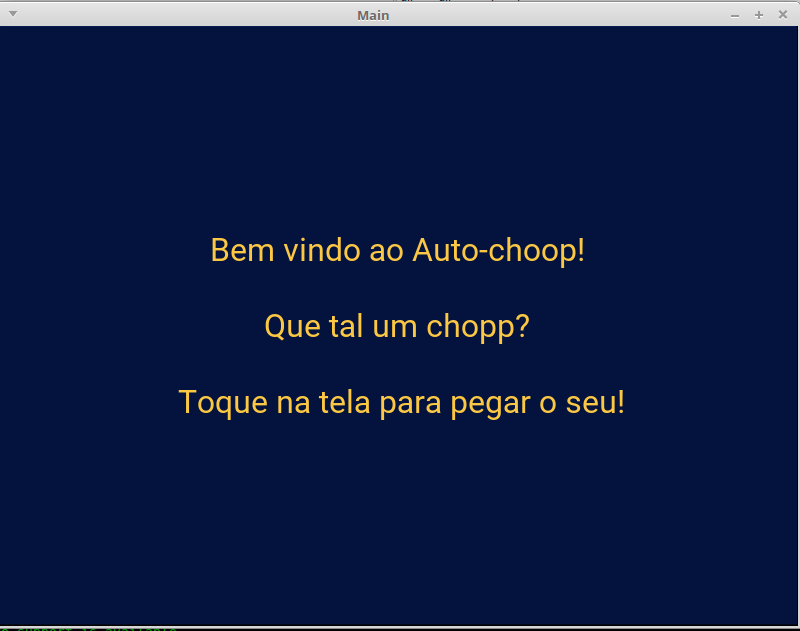
\includegraphics[scale= 0.4]{figuras/home-screen.png}
            \caption{Tela Inicial. Fonte: Própria.}
            \label{home-screen}
        \end{figure}

        \begin{figure}[H]
            \centering
            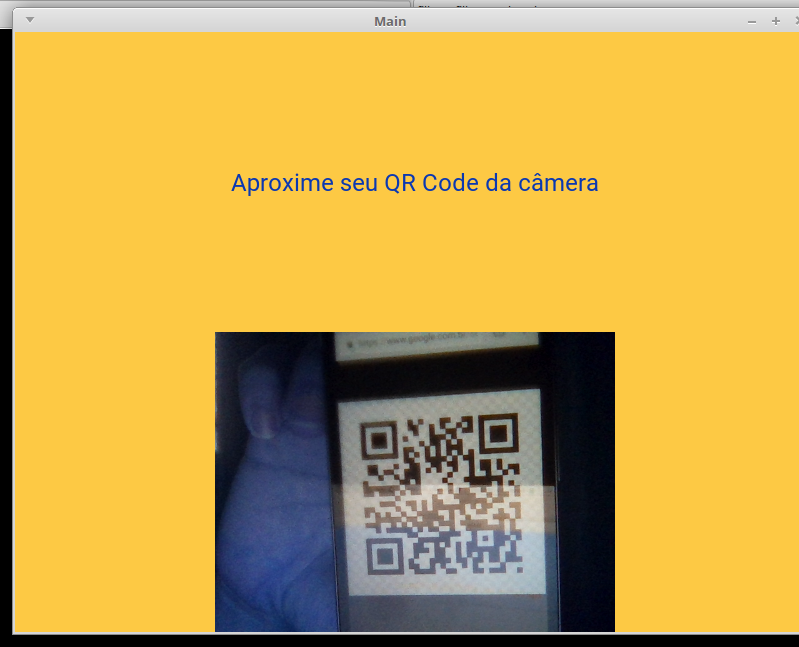
\includegraphics[scale= 0.4]{figuras/leitor-qrcode.png}
            \caption{Tela de Leitura de \textit{QRCode}. Fonte: Própria.}
            \label{leitor-qrcode}
        \end{figure}

        \begin{figure}[H]
            \centering
            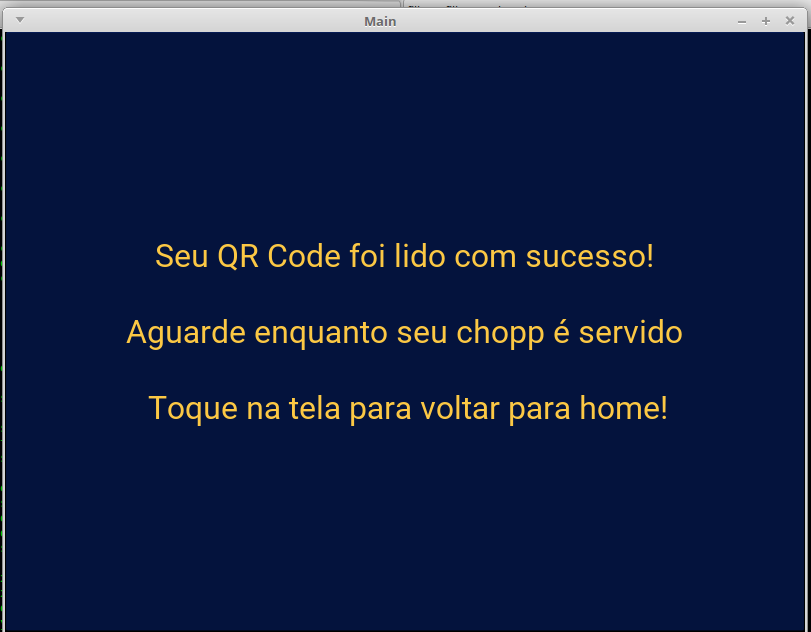
\includegraphics[scale= 0.4]{figuras/sucesso.png}
            \caption{Tela informando que o \textit{QRCode} foi lido com sucesso. Fonte: Própria.}
            \label{sucesso}
        \end{figure}

        \begin{figure}[H]
            \centering
            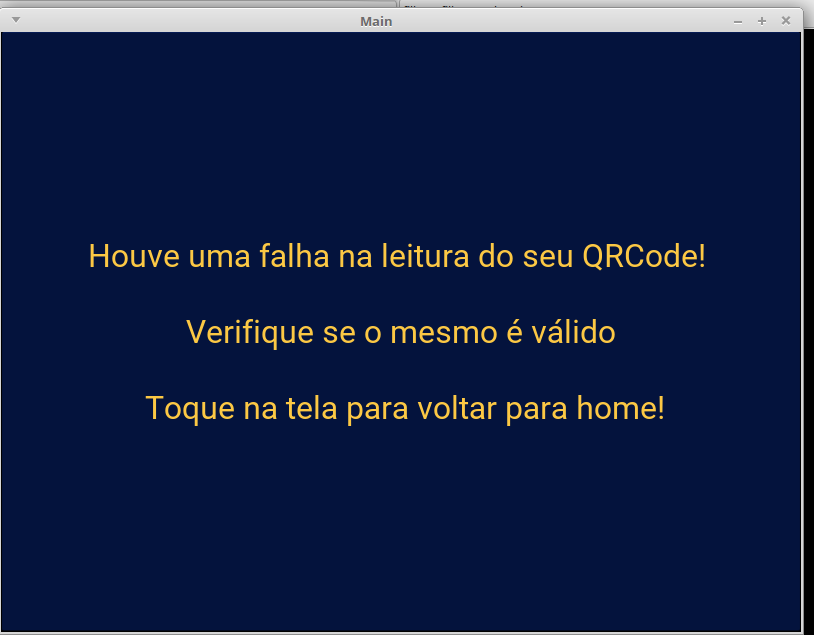
\includegraphics[scale= 0.4]{figuras/falha.png}
            \caption{Tela informando que o \textit{QRCode} não foi lido com sucesso. Fonte: Própria.}
            \label{falha}
        \end{figure}
    
        
